\section[The cooking]{USB stick preparation}
\subsection{Ingredients}
\begin{frame}{USB recipe, ingredients}
  \begin{description}[short]
  \item[Distribution] Ubuntu based host OS.
    \begin{itemize}
    \item Up to date kernels, more chance to use with new laptops.
    \item Otherwise quite stable
    \item Start with \Code{ubuntu-mini-remix-14.04.1-amd64.iso} from
      \url{http://www.ubuntu-mini-remix.org/}
    \item Use lightweight desktop like XFCE4.
    \item Current version 14.04.1 LTS.
    \end{itemize}
  \item[Apps]  Mix and match whatever you need. Most of the time with a
    simple \Code{apt-get install} sometimes special PPAs (e.g. Java 8).
  \item[Home grown packages] Maybe some deb [re]packaging required:
    Netbeans, glassfish etc.\\
    Packaging is simple: Pickup an installed version of the app, add some meta
    info and checksum the lot. See script sample.
  \end{description}
\end{frame}

\subsection{Tools}
\begin{frame}{USB recipe, Tools}
  \begin{description}[short]
  \item[Host] computer running same OS version. This eases work.\\
    Tweak
    the max number of boot devices (add a parameter to grub command line).
  \item[Customizer] Simple but adequate. Version 3.2.3.
    \begin{itemize}
    \item Needs some tweaks to get it running. (Gambas 3 vs 2 on U 14.04).
    \item \url{https://github.com/clearkimura/Customizer}.
    \item Revived. They seem to be moving to python.
    \end{itemize}
  \item[Startup Disk Creator] (\Code{/usr/bin/usb-creator-gtk}),
    standard in Ubuntu.
  \item[DD] Good old \Code{dd}.
  \item[Cook] A good Linux Cook\InlineSmiley. Some knowledge is indispensable.
  \end{description}
\end{frame}

\subsection[Stir well]{Stir well}
\begin{frame}{Preparing the dough}
  \begin{columns}
    \begin{column}{.6\textwidth}
      \begin{itemize}
      \item Prepare basic stick.
        \begin{itemize}
        \item Load iso file with customizer. This will unpack iso into
          \Code{/home/FileSystem} and live system helpers into \Code{/home/ISO}
        \item Open \Okis{terminal} in customizer. This does 'apt-get
          update' automatically. 
        \end{itemize}
      \end{itemize}
    \end{column}
    \begin{column}{.4\textwidth}
      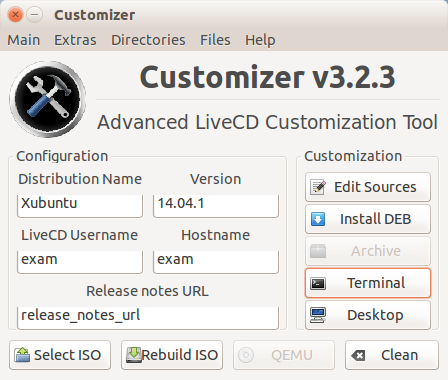
\includegraphics[width=\textwidth]{figures/customizer.png}
    \end{column}
  \end{columns}
  \begin{itemize}
  \item In the terminal you have all apt-tools. You are in a \Code{chrooted} environment
  \item Install (apt-get) whatever you want, e.g. desktop and window manager
    (e.g. XFCE4) and any apps you like.
  \item Install local \Code{.deb} packages with 'install deb
    package'.
  \item Rebuild ISO which creates a new iso file in \Code{/home/}.
  \item Rename the iso, e.g. add a date to it. This ISO is also a
    snapshot, making it easy to revert your steps.
  \end{itemize}
\end{frame}

\begin{frame}{Make a sticky}
  \begin{itemize}
  \item Add exam user account and settings (e.g. 'empty password').
  \item Add correctors account if required.
  \item Add everything you need in the next steps to the
    \Code{/home/FileSystem}. That will land in the ISO and stick too.\\
    Example: JDK documentation for on stick browsing during exam.
  \item Bake one stick first. Simply use \textbf{Startup Disk Creator} from the
    Host menu. Allow for some work space. 1GB (the default) is
    typically just fine.
  \item Test it.
  \item If satisfying, continue to the next step, otherwise do some more
    tweaking in customizer as required.
  \item You could provide the ISO to the students, so they can
    practice with the USB and IDE on their device. I offered to
    create (batches) of sticks, owned by the students.
  \end{itemize}
\end{frame}

\subsection[EXAM proof]{Making it exam proof}
\begin{frame}{Make it exam proof}
  \begin{itemize}
  \item Remove add kernel modules and drivers not needed.
    \begin{itemize}
    \item Network\footnote{You can leave wired network in, if you want
      a network based exam}, wifi, bluetooth, local hard drives.
    \end{itemize}
  \item Remember to do a \Code{depmod} -a inside the
    \textbf{customizer-terminal}. Otherwise your stick will not boot.
  \item Make a new ISO. Rename it properly.
  \item Test again of course.
  \end{itemize}
\end{frame}

\lstset{basicstyle={\scriptsize}}
\subsection[Production]{Prime for Production}
\begin{frame}{Prepare exam workspace}

  \begin{itemize}  \item Bake a new stick and boot from it on exam machine to \textit{prime} it. This
    will create the exam user space under \Code{/exam/exam}.
  \item Tweak settings and such (UI menu to make it less confusing,
    remove unneeded desktop icons, make browser bookmarks to local
    documentation, e.g. to JDK doc.
  \item Shut down exam test machine.
  \item Mount the primed stick with 
    \lstinputlisting[language=sh]{code/scripts/casper-simple-example}
  \item Save the primed data \Okis{exam work space} from \Code{exam/exam} to some place safe
    for later use (stick cleanup). Use e.g. \Code{tar czf} or
    zip. Result: \Code{skell.tgz}
\end{itemize}
\end{frame}

\subsection[Baking]{Baking sticks in batches}
\begin{frame}[shrink]{Stir, bake at 5 Volts, 14 per batch}
  \begin{itemize}
  \item Make a \Code{dd}-copy of the primed stick and save it under a
    {\ttfamily\textbf{proper-name}.img}
    \lstinputlisting[language=sh]{code/scripts/dd-read-master}
  \item (sticky) Label your sticks if you not already did so.
  \item Now connect your USB hubs and
  \item Insert your sticks, ensuring the host sees it. (as in: wait a
    bit between sticks).
  \item Insert in label
    order. In this phase it ensures proper matching of stick label and
    stick disk-label (EXAM101).
  \item start the \Code{mkExamSticks} script with appropriate parameters
    \lstinputlisting[language=sh]{code/scripts/mksticks-example}
    This writes and labels all 14 sticks (the c parameter) in \textit{parallel},
    which takes about 90 seconds on my machine.
  \end{itemize}
\end{frame}

\begin{frame}{Core of bake script}
The speed-up lies in the way you start \Code{dd} sub processes and the extra
parameters to dd.
\lstinputlisting[firstline=72,lastline=90,language=sh,basicstyle={\tiny},%
caption={Tiny details count here},morekeywords={conv,fsync}]{code/scripts/mkExamSticks}
\end{frame}

\begin{frame}{The topping, the exam tasks}
  \begin{itemize}
  \item In our setup, the students receive a stick, personalized, with
    the appropriate netbeans project pre installed in
    \Code{/exam/exam/Desktop/examproject} or similar.
  \item We prepare the exam from a solution project
    \begin{itemize}
    \item adding corrector tags and TODO tags (manual labor).\\
      Here the corrector's workbench Netbeans plugin might be handy.
    \item strip the solution
    \item Make personalized copies with one copy per stick
      (e.g. EXAM101), this is the \Okis{local sandbox}.
    \item Put them in a repository, one per student, if you so require.
    \end{itemize}

  \item Insert the sticks in the hubs, connected, the disk label now identifies the sticks.
  \item Use the \Code{primeSticks} command, no parameters; it can find
    how many sticks are mounted.
    \begin{itemize}
    \item Installs fresh copy of the exam work space.
    \item rsyncs local sandbox into exam work space.
    \end{itemize}
  \end{itemize}
\end{frame}

\begin{frame}{The proof is in the eating}
  \begin{itemize}
  \item Take the exam.
  \item Collect the sticks.
  \item \textit{Harvest} the student projects.
    \begin{itemize}
    \item Insert the sticks into the hubs
    \item use the command \Code{harvestSticks} to rsync the exam stuff
      back into the local sandbox.
      \begin{itemize}
      \item Takes about 20 seconds for 14 sticks.\\
      \item Inserting and removing sticks takes about the same time.
    \item With 2 pairs of hubs your could speed up even a bit more.
    \end{itemize}
  \item Commit the work into the repository.
  \end{itemize}
  \item Make the exam work available to the correctors.
    \begin{itemize}
    \item Not netbeans plugin here yet\InlineMwha.
    \item Now using simple PHP based web app, to allow parallel
      corrections by multiple correctors
    \end{itemize}

  \end{itemize}
\end{frame}

